\documentclass[sigconf]{acmart}

\usepackage{algorithm}
\usepackage{algpseudocode}% http://ctan.org/pkg/algorithmicx
\algrenewcommand\algorithmicrequire{\textbf{Input:}}
\algrenewcommand\algorithmicensure{\textbf{Output:}}
\usepackage{hyperref}
\usepackage{bbold}
\usepackage{enumitem}
\usepackage{graphicx}
\usepackage{bm}
\usepackage{animate}

\begin{document}

\title{COMP6247 - Final Assignment}
\author{Luke McClure \\ lam3g17@soton.ac.uk \\ 29573904}

\maketitle

\section{Part I: Radial Basis Functions}
I chose the Istanbul Stock Exchange dataset\footnote{https://archive.ics.uci.edu/ml/datasets/ISTANBUL+STOCK+EXCHANGE} to experiment with RBF regression with.
\subsection{RBF Regression}
RBF models aim to replicate neural networks without the massive complications of training, this is achieved by capuring non-linear properties with linear parameters through fixing of many of the paramaterisable options.
A singular RBF will calculate a nonlinear distance through a function, and these functions form a weighted sum to achieve a result.
An RBF model of J basis functions takes the form:
\begin{equation}
  f(\mathbf{x}) = \sum^J_{j=1}w_j\phi(||\mathbf{x}-\mathbf{m_j}||/\sigma_j)
\end{equation}

By creating a N x J "design matrix" U with matrix elements given using the equation below we can transform the RBF problem into a least squares problem, allowing us to form a closed form solution for the optimum weights.

\begin{equation}
  u_{ij}=\phi(||\mathbf{x_i}-\mathbf{x_j}||/\sigma_j), i=1,...,N, j=1,2,...,J
\end{equation}

\begin{equation}
  \mathbf{w} = (U^TU)^{-1}U^T\mathbf{y}
\end{equation}

\begin{figure}[h]
  \centering
  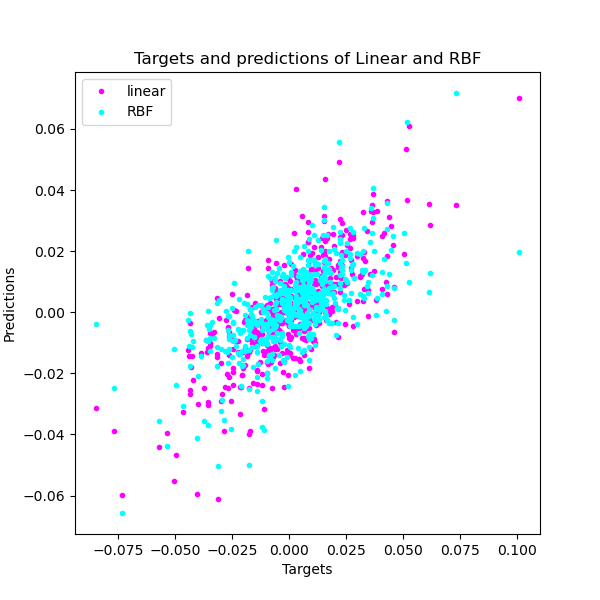
\includegraphics[scale=0.35]{../RBF-R/CF.png}
  \caption{Comparison of predictions between closed form linear and RBF regression}
  \label{fig:CF}
\end{figure}

Closed form solutions are not particularly helpful if we do not have the targets at hand such as in the later portions of this coursework, in this case Stochastic Gradient Descent is necessary in order to gradually converge onto the same optimal solution that can be found using the closed form equation.

\begin{equation}
  \mathbf{w_{t+1}} = \mathbf{w_t} + \alpha[y_t - f(\mathbf{x_t}, \mathbf{w_t})]\nabla f(\mathbf{x_t}, \mathbf{w_t})
\end{equation}

This is used starting with a random set of weights to gradually learn the weights with a fixed learning rate of $1e^{-2}$.

Whilst 10,000 iterations is a conventionally very high running time for this sort of problem, the RBF representation has not converged with the optimal weights learned from the closed form solution.

  \begin{figure}
    \centering
    \begin{minipage}{.3\textwidth}
      \centering
      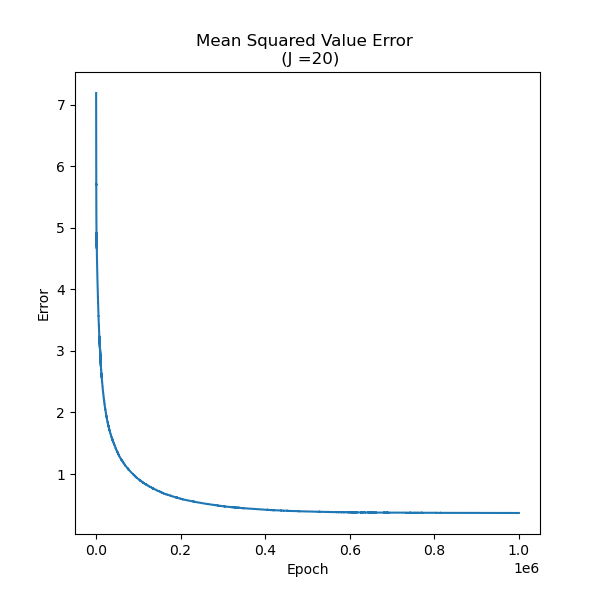
\includegraphics[width=.8\linewidth]{../RBF-R/LOSS-1000000.png}
      \captionof{figure}{Error curve}
      \label{fig:LOSS1000000}
    \end{minipage}%
    \begin{minipage}{.3\textwidth}
      \centering
      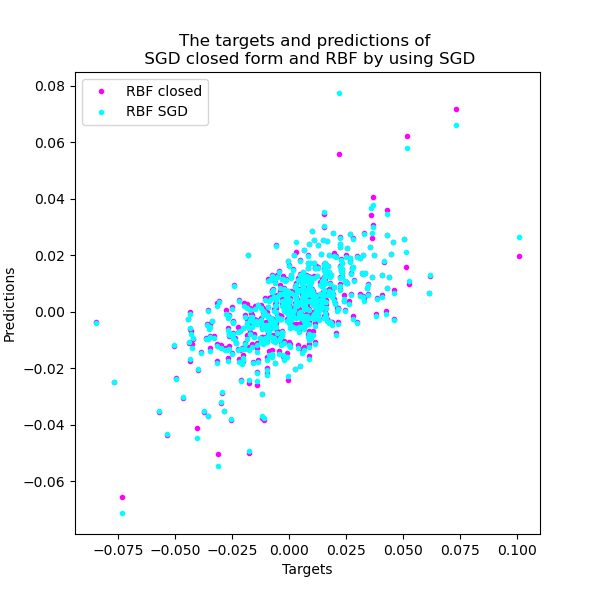
\includegraphics[width=.8\linewidth]{../RBF-R/SGD-1000000.png}
      \captionof{figure}{Prediction plot}
      \label{fig:SGD1000000}
    \end{minipage}
    \begin{minipage}{.3\textwidth}
      \centering
      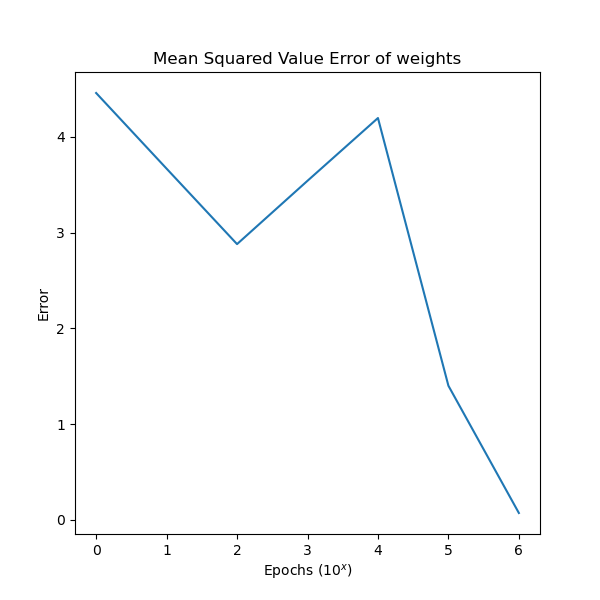
\includegraphics[width=0.8\linewidth]{../RBF-R/LWEIGHTS.png}
      \caption{MSE between weights of close form and SGD RBF}
      \label{fig:LWEIGHTS}
    \end{minipage}
  \end{figure}

By running SGD for much longer it is clear from \autoref{fig:SGD1000000} that after 1,000,000 iterations SGD is able to converge successfully on to the optimal weights learned from the close form representation of the problem.
\autoref{fig:LWEIGHTS} shows how the MSE between the optimal weights and the weights learned from SGD change as the number of iterations increases, eventually closing in to an MSE of almost 0 indiciating an optimal solution.

\subsection{Mountain Car using RBF}
\subsubsection{Tabular Discretization with RBF approximator}

We are able to generate a Q-table to solve the classic Mountain Car problem by quantizing the space into 40 steps along each axis and building this table to measure the 'value' of each move within the action space at each state.

The Q values within this Q-table are iteratively changes through steps, this alters the current Q value according to a scaled reward at the current state and a time difference between the Q value for the current state and the next according to the best action to take.
\begin{equation} \label{eqn:Qtab}
  Q(S_t, A_t) \leftarrow Q(S_t, A_t) + \alpha [R_{t+1} + \gamma \max_a Q(S_{t+1}, a) - Q(S_t, A_t)]
\end{equation}

The animation of \autoref{anim:Qtab} shows the Q table being built up over 300 episodes for each state within the position-velocity grid the car is bounded within. 
\autoref{anim:Qtab} shows clearly how the Q-table becomes more accurate as more episodes are performed, it is natural to assume this continues until the Q-table represents the real world cost function as accurately as can be stated within the confines of quantization.
\begin{figure}[h]
  \centering
  \animategraphics[scale=0.30,autoplay,loop]{30}{../MCar/anim/Q_table_e_}{0}{299}
  \caption{Tabular building of Q Table (animation)}
  \label{anim:Qtab}
\end{figure}

\autoref{fig:1KEpisode} shows the trained Q-Table after 1000 episodes, with the algorithm largely settling into the optimal action values for each state. 
The number of steps for each episode is represented in \autoref{fig:STEPS}, showing how after a few very long episodes at the start of training the algorithm settles into using a very consistent amount of steps.
This could be as most of the training process has already been completed and the car will be mostly performing the same actions in order to complete task, rather than exploring through new states.

\begin{figure}
  \begin{minipage}{.5\textwidth}
    \centering
    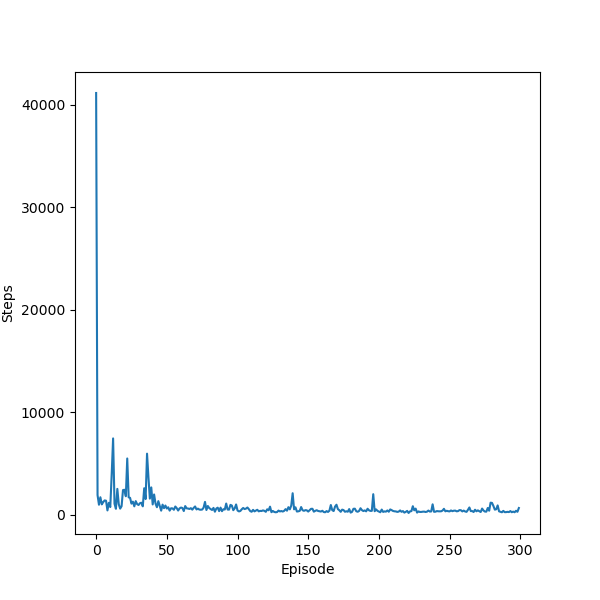
\includegraphics[width=.6\linewidth]{../MCar/STEPS.png}
    \captionof{figure}{Measure of steps per episode}
    \label{fig:STEPS}
  \end{minipage}%
  \begin{minipage}{.5\textwidth}
    \centering
    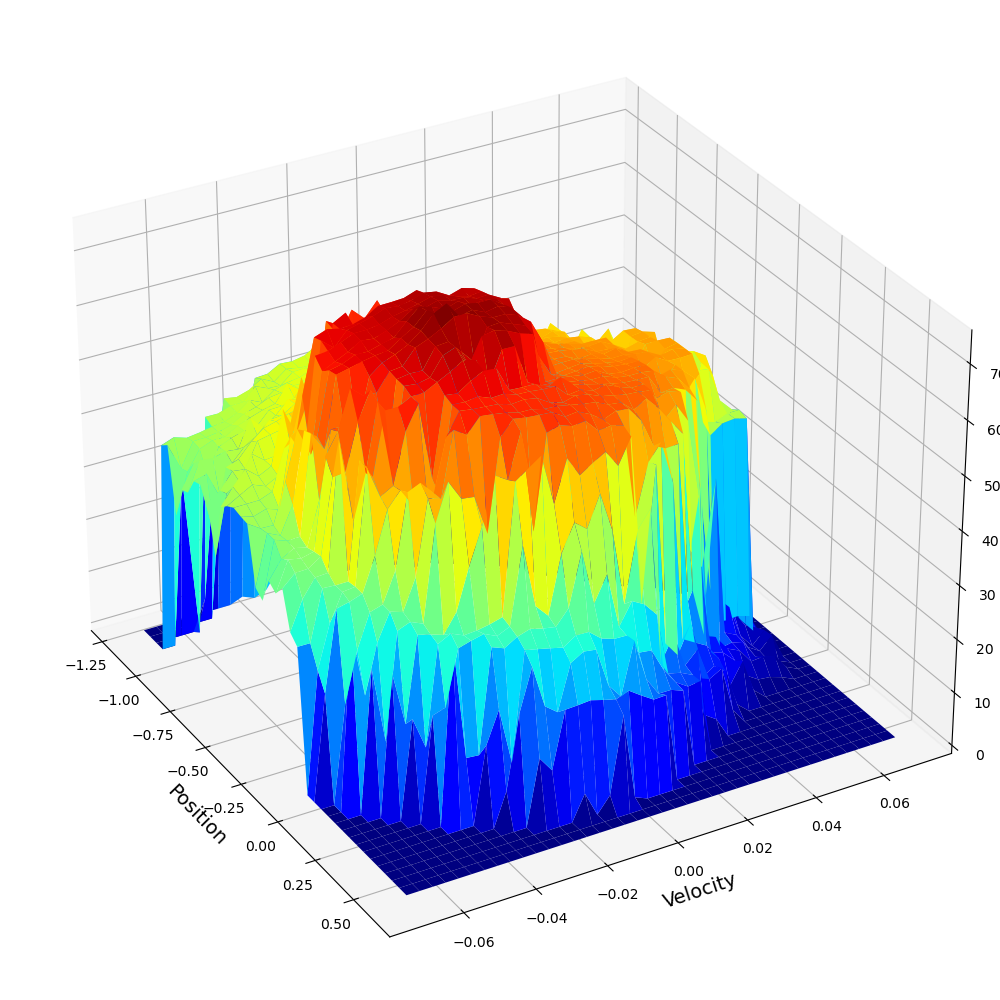
\includegraphics[width=.6\linewidth]{../MCar/1000 Episode.png}
    \captionof{figure}{Q table after 1000 episodes}
    \label{fig:1KEpisode}
  \end{minipage}
\end{figure}
A Q-Table is unwieldy and large in high dimension state and action spaces, it is much more space efficient to try and learn the Q-Table using the functional approximation RBF. 
By using kmeans to find the centre of clusters within the state space we can make the RBF a lot more efficient by focusing more attention to areas in the state space with a higher complexity, 
this does not particularly apply for the uniform state space constructed in the Mountain Car problem but can still be applied.

With any functional approximation there will inherently be errors, \autoref{fig:JErrors} is the measure of error in the approximation compared to the 1000 episode Q-Table previously shown. 
As more basis functions are added the functional appriximation is able to more accurately represent the finer details within the state space. 
In terms of RBF specifically a higher number of cluster centres means that there is more chance of every detail within the confined state space being captured.

Testing to ensure the RBF approximation yields successful end states and measuring the number of steps to complete the puzzle generates \autoref{fig:JSteps}. 
While the number of basis features affects the error compared to the original Q-Table all approximations are able to complete the task in a relatively comparable amount of time.
\begin{figure}
  \begin{minipage}{.45\textwidth}
    \centering
    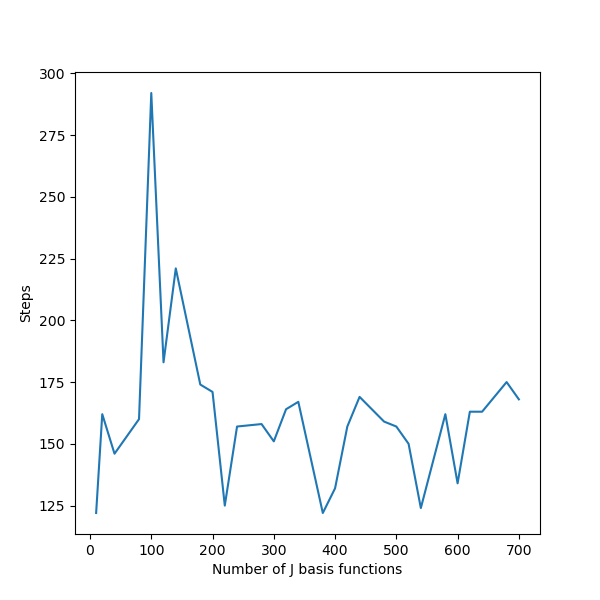
\includegraphics[width=.6\linewidth]{../MCar/JSteps.png}
    \caption{Measure of steps completed}
    \label{fig:JSteps}
  \end{minipage}
  \begin{minipage}{.45\textwidth}
    \centering
    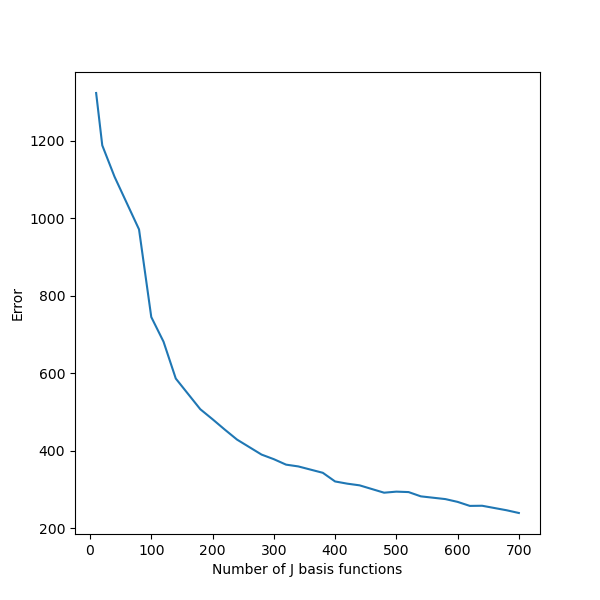
\includegraphics[width=.6\linewidth]{../MCar/JErrors.png}
    \caption{Error of RBF approximation}
    \label{fig:JErrors}
  \end{minipage}
\end{figure}

\subsubsection{Online Learning of RBF}
Functional approximation frees up a lot of space from the memory ineffient method of Q-Tables, and proving we are able to approximate the Q-Table using these functional approximations is an important stage.
To streamline the process into learning the weights for the functional approximation is an important next stage to take that will free up the memory intensive first stage from the previous section.

The SARSA method of learning the Q-Space in an efficient way can be paired with stochastic gradient descent in the more typical sense for classic supervised learning. 

The weights for (in this case the RBF function) would be learned using \autoref{eqn:SARSA} at each step, with the weight being altered by the learning rate times the immediate reward plus the Time Difference reward.
This is all multiplied by the differential of the q function with respect to the weights in order to descent down the gradient.

\begin{equation} \label{eqn:SARSA}
  w \leftarrow w + \alpha[R_t +\gamma \hat{q}(S', A', w) - \hat{q}(S, A, w)]\nabla \hat{q}(S, A, w)
\end{equation}

My implementation suffers from issues with exploding weights, resulting in infinity's being encountered in training and the algorithm being unable to complete.

The only plot able to be drawn from this learning was \autoref{fig:SARSA} with J=5 and over 5 episodes. While this is not representative of the ability for this algorithm to learn fully, the semi destictive shape
of the Q-Table can somewhat be seen, even if the low number of basis functions render it in very low quality.

\begin{figure}[h]
  \centering
  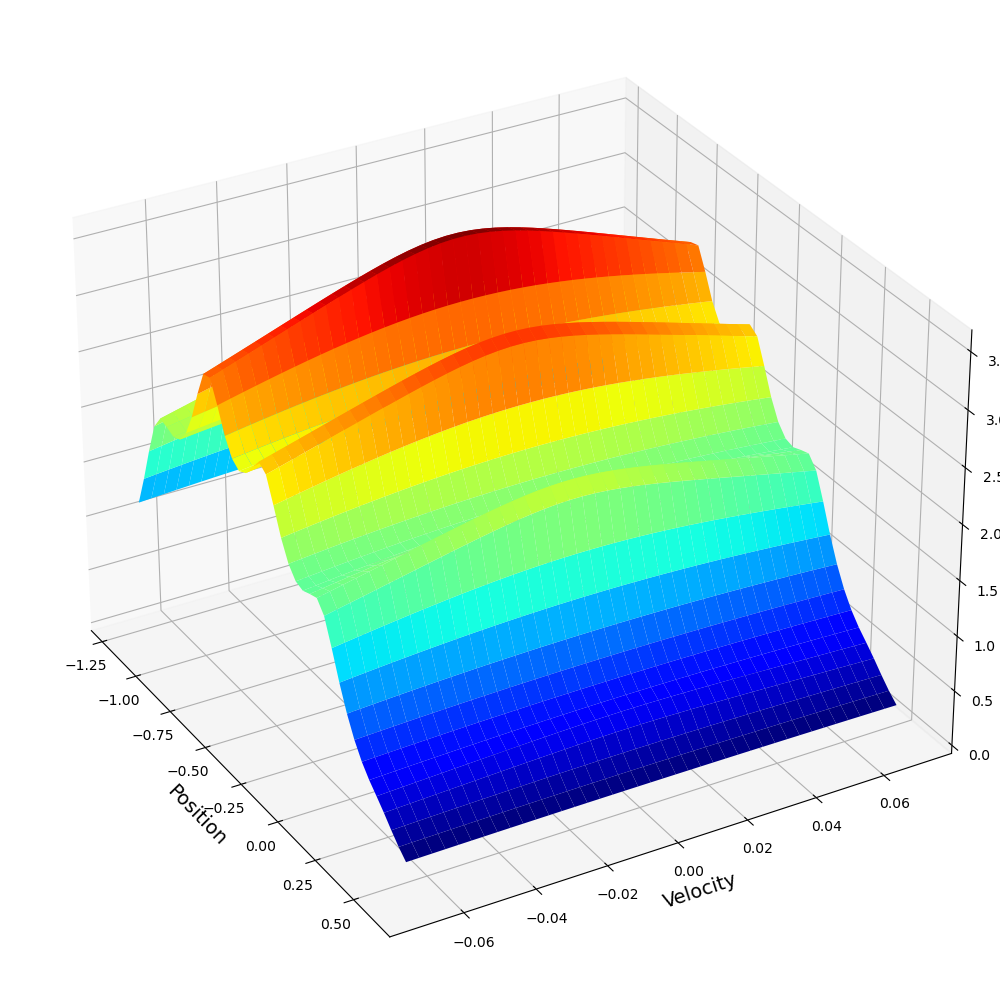
\includegraphics[scale=0.2]{../MCar/SARSAanim/SARSA_RBF_e_2.png}
  \caption{Online RBF Q-Table}
  \label{fig:SARSA}
\end{figure}

\subsection{Adaptive RBF}

While fixing the RBF functional approximator's number of basis functions (J) has been done manually up until now, handing this control over to the automation would benefit in both effort taken to tune the network as well as 
the potential overall accuracy of the system. 
A method to do this has been outlined in the work by John Platt \cite{RAN}, which forms a basis in trying to understand types of patterns that are well understood by the network.

If the network understands that there are patterns being seen that are not well understood by the neurons of the network already then it has the capacity to generate a new neuron in order to capture this new pattern that has been previously unseen.
This is achieved by comparing inputs to asssigned gaussian centres that represent already known patterns. If the error of the network output exceeds a certain threshold $e_{min}$ and the input is further than an assigned distance $\epsilon$ then a new basis function and centroid will be created to depict this pattern.
If these conditions are not met then the weights are altered as per normal gradient descent.

In practicality this means using the RAN algorithm with the RBF network we could set the intial number of basis functions $J$ to be a very low number and let the network decide when a new basis function is needed to capture new scope within the input-output space.
However this also requires several more hyperparameters $\epsilon_{max}$ and $\gamma$ to be set.
\begin{algorithm}
  \caption{Learning RBF weights using RAN}
  \begin{algorithmic}
    \Require Input-output pairs=$(x,y)$ from Q-learning
    \Ensure Weights $w$ of RBF function
    \State {$f(x) = \sum^{K}_{\kappa=1}\alpha_\kappa \phi_\kappa (x)$}
    \State {$\phi_\kappa(x) = \exp(-(\frac{||x-c_k||}{\sigma_\kappa})^2)$}
    \State {$\epsilon_n = \epsilon_{max}$}
    \ForAll {$(x, y)$ in pairs}
    \State {$\epsilon_n = max(\gamma^n\epsilon_{max}, \epsilon_{min})$}
    \State {$e_n = y - f(x)$}  
    \State {$d = min_n||c_n - x||$}
    \If {$e_n > e_{min}$ and $d >\epsilon_n$}
    \State {$\alpha_{\kappa+1} = e_n$}
    \State {$c_{\kappa+1} = x$}
    \State {$\sigma_{\kappa+1}=\kappa d$}
    \Else 
    \State {$w_{n+1} = w_{n} + \eta e_n \nabla_w f(x)$}
    \EndIf
    \EndFor
  \end{algorithmic}
\end{algorithm}
\section{Part II: Summarising a recent scientific study}
I will be summarising a work on using RL to optimize neural nets\cite{li2017learning}.
\subsection{Summary}
When training a neural network a lot of computational and human time and effort is put into optimising the hyperparameters of a neural net such as fiddling with learning rates, optimisation functions, attempting to navigate loss landscapes.
The idea behind this paper is to be able to find a generalised policy that is able to make changes to the process of training a network on the fly to dramatically increase the efficiency of this training process.
Ideally this policy should be able to recognise trends within the domain of training neural networks and be able to adjust the training parameters such that the trained network is able to perform optimally with minimal training.
  
This problem was supposed to be solvable with reinforcement learning due to a number of key observations about the nature of training neural nets.
The best indicator that this problem could be solved by RL is noticing how ML engineers/researchers will train a neural network classically. The typical process involves a lot of watching how the loss curve behaves and monitoring accuracy for overfitting and then altering parameters to improve these scores.
This basic summary of how neural nets are trained sounds very like the domain of RL, with an environment to be monitored, values to change and a score to be fed back from this environment.

The fact that people who are experienced with neural networks start to get a feel for how a network can behave and can start to build up an intuition of how a network may react also flags the idea that this sort of problem is not iterative guesswork but can be learnable through experiencing the problem, something RL methods excel at.
This learnable experience hints that there are common factors that can be learned when trying to train neural networks, this paper aims to try exploit this.
\subsection{Reinforcement Learning Formulation}
To create a Reinforcement Learning problem several key areas must be defined:
\begin{itemize}
  \item States\\
  States within this problem are defined as the current iterate $x^{(t)}$ and features $\Phi(\cdot)$. These features include the history of iterates $x^{(1)},...,x^{(T)}$, gradients $\nabla \hat{f}(x^{(1)}),...,\nabla \hat{f}(x^{(T)})$, and objective values $\hat{f}(x^{(1)}),...,\hat{f}(x^{(T)})$.
  The last few steps within all of these features of $\Phi(\cdot)$ are averaged to produce a singular value of each for the state and to denoise some of these values (particularly the gradients and objective values).
  These capture the entire domain of the current output of functions, the loss of these functions and the gradients of these losses which are all important in determining how the learning parameters may be affecting training.
  
  With these in mind a state value $s_t = (x^{(t)}, \Phi(\cdot))^T$.
  \item Actions\\
  An action within this model $a_t$ is the learning rate of the neural net, otherwise stated as the step size $\Delta x$ used to update the iterate. 
  \item Observations\\
  An observation made by this model simply consists of the features $\Phi(\cdot)$ as well as the previous memory state of the learned optimization algorithm.
  This previous memory state takes the form of a recurrent neural net and is described as a statistic of the prvious observations that is learned jointly with the policy.

  \item Rewards\\
  This method does not use an explicit reward to maximise when learning the function, but rather a cost to minimize basis of deriving the worth of a state.
  The explicit cost minimization function is not explicitly defined but instead left general for an optimization algorithm $A^*$ being:
  \begin{equation}
    \mathbb{E}_{f\sim F,x^{(0)}\sim D}[L(f,A^*(f,x^{(0)}))]
  \end{equation}
  The paper then assumes that we would like to minimize the objective function, given the nature surrounding the paper.
  The model is defined to attempt to minimize the area under the loss curve during training of a function, therefore having the knock on effect of making the 
  training gradient much sharper and both reducing the time to converge and the objective function.

  To minimise this area under the loss curve the meta-loss is defined as:
  \begin{equation}
    \sum_{i=1}^Tf(x^{(i)})
  \end{equation}
  \item Policy models\\
  The overall goal of this paper is to learn a policy that will minimise the expected total cost over time, which in the case for training neural networks is measured in epochs.

  The optimal action policy is strictly defined as:
  \begin{equation}
    \pi^* = \arg\min_\pi \mathbb{E}_{(s_0,a_0),(s_1,a_1),...,(s_T,a_T)}\sum_{t=0}^{T}c(s_t)
  \end{equation}

  The policy generating any action is defined as:
  \begin{equation}
    \pi(a_t|o_t, t) = \mathit{N}(\mu^\pi(o_t),\Sigma^\pi(o_t))
  \end{equation}
  The curious aspect of this paper is that both the parameters that the normal distribution that samples a policy are modelled by neural networks themselves with the observations as an input.

\end{itemize}
\subsection{Learning Paradigm}
  The use of neural networks to form the basis of the action policy hinders the simplicity in learning learning it, meaning that the policy itself is not directly learnable as instead we must train the two neural nets that supply the policy distribution.
  
  To solve this problem the researchers resorted to Guidance Policy Search in order to learn these complex weights. During each iteration a policy optimation will be performed on $\Psi$ which uses the resultant policy in supervised training of $\pi$.
  This is conducted by performing a relaxed constraint optimisation problem to solve an equality of the expectations $\Psi$ and $\pi$.
  \begin{equation}
    \min_{\theta, \eta}\mathbb{E}_{\Psi}[\sum^{T}_{t=0}c(s_t)] s.t. \mathbb{E}_{\Psi}[a_t]=\mathbb{E}_{\Psi}[\mathbb{E}_{\pi}[a_t|s_t]]\forall t
  \end{equation}
  
  ADMM is used to perform this relaxed constrained optimisation, the basic idea of ADMM is to work on the minimisation of one argument at a time. 
  The algorithm works through each argument pinning found minimums at their values while working on the next.
\subsection{Significance and future influence}
The conclusions of this paper are very interesting, showing promising results that this method is robust to both architecture changes and different datasets than originally trained with.
There is a clear steeper error curve with the models trained using this method than with several other common optimisers, and even another method that is similar in goals to this one. 

The generalisation that is shown in the results shows how using an RL style ... can learn properties of training neural networks and was successful in the goals of the paper.
With several datasets being used and multiple different optimisers including one of a similar concept being used to compare the results of this paper hold up to some level of scrutiny, and shows this 
method could be utilised effectively into the future. 

This method may not be of massive benefit to research implicitly in the short term, but the ability to train networks efficiently could be a massive in business applications where resources are a key factor in weighing up a project.

\bibliography{refs}
\bibliographystyle{plain}
\end{document}
\endinput